\documentclass[]{article}
\usepackage{lmodern}
\usepackage{amssymb,amsmath}
\usepackage{ifxetex,ifluatex}
\usepackage{fixltx2e} % provides \textsubscript
\ifnum 0\ifxetex 1\fi\ifluatex 1\fi=0 % if pdftex
  \usepackage[T1]{fontenc}
  \usepackage[utf8]{inputenc}
\else % if luatex or xelatex
  \ifxetex
    \usepackage{mathspec}
  \else
    \usepackage{fontspec}
  \fi
  \defaultfontfeatures{Ligatures=TeX,Scale=MatchLowercase}
\fi
% use upquote if available, for straight quotes in verbatim environments
\IfFileExists{upquote.sty}{\usepackage{upquote}}{}
% use microtype if available
\IfFileExists{microtype.sty}{%
\usepackage{microtype}
\UseMicrotypeSet[protrusion]{basicmath} % disable protrusion for tt fonts
}{}
\usepackage[margin=1in]{geometry}
\usepackage{hyperref}
\hypersetup{unicode=true,
            pdftitle={Component-wise Boosting with compboost},
            pdfauthor={Daniel Schalk},
            pdfborder={0 0 0},
            breaklinks=true}
\urlstyle{same}  % don't use monospace font for urls
\usepackage{color}
\usepackage{fancyvrb}
\newcommand{\VerbBar}{|}
\newcommand{\VERB}{\Verb[commandchars=\\\{\}]}
\DefineVerbatimEnvironment{Highlighting}{Verbatim}{commandchars=\\\{\}}
% Add ',fontsize=\small' for more characters per line
\usepackage{framed}
\definecolor{shadecolor}{RGB}{248,248,248}
\newenvironment{Shaded}{\begin{snugshade}}{\end{snugshade}}
\newcommand{\KeywordTok}[1]{\textcolor[rgb]{0.13,0.29,0.53}{\textbf{#1}}}
\newcommand{\DataTypeTok}[1]{\textcolor[rgb]{0.13,0.29,0.53}{#1}}
\newcommand{\DecValTok}[1]{\textcolor[rgb]{0.00,0.00,0.81}{#1}}
\newcommand{\BaseNTok}[1]{\textcolor[rgb]{0.00,0.00,0.81}{#1}}
\newcommand{\FloatTok}[1]{\textcolor[rgb]{0.00,0.00,0.81}{#1}}
\newcommand{\ConstantTok}[1]{\textcolor[rgb]{0.00,0.00,0.00}{#1}}
\newcommand{\CharTok}[1]{\textcolor[rgb]{0.31,0.60,0.02}{#1}}
\newcommand{\SpecialCharTok}[1]{\textcolor[rgb]{0.00,0.00,0.00}{#1}}
\newcommand{\StringTok}[1]{\textcolor[rgb]{0.31,0.60,0.02}{#1}}
\newcommand{\VerbatimStringTok}[1]{\textcolor[rgb]{0.31,0.60,0.02}{#1}}
\newcommand{\SpecialStringTok}[1]{\textcolor[rgb]{0.31,0.60,0.02}{#1}}
\newcommand{\ImportTok}[1]{#1}
\newcommand{\CommentTok}[1]{\textcolor[rgb]{0.56,0.35,0.01}{\textit{#1}}}
\newcommand{\DocumentationTok}[1]{\textcolor[rgb]{0.56,0.35,0.01}{\textbf{\textit{#1}}}}
\newcommand{\AnnotationTok}[1]{\textcolor[rgb]{0.56,0.35,0.01}{\textbf{\textit{#1}}}}
\newcommand{\CommentVarTok}[1]{\textcolor[rgb]{0.56,0.35,0.01}{\textbf{\textit{#1}}}}
\newcommand{\OtherTok}[1]{\textcolor[rgb]{0.56,0.35,0.01}{#1}}
\newcommand{\FunctionTok}[1]{\textcolor[rgb]{0.00,0.00,0.00}{#1}}
\newcommand{\VariableTok}[1]{\textcolor[rgb]{0.00,0.00,0.00}{#1}}
\newcommand{\ControlFlowTok}[1]{\textcolor[rgb]{0.13,0.29,0.53}{\textbf{#1}}}
\newcommand{\OperatorTok}[1]{\textcolor[rgb]{0.81,0.36,0.00}{\textbf{#1}}}
\newcommand{\BuiltInTok}[1]{#1}
\newcommand{\ExtensionTok}[1]{#1}
\newcommand{\PreprocessorTok}[1]{\textcolor[rgb]{0.56,0.35,0.01}{\textit{#1}}}
\newcommand{\AttributeTok}[1]{\textcolor[rgb]{0.77,0.63,0.00}{#1}}
\newcommand{\RegionMarkerTok}[1]{#1}
\newcommand{\InformationTok}[1]{\textcolor[rgb]{0.56,0.35,0.01}{\textbf{\textit{#1}}}}
\newcommand{\WarningTok}[1]{\textcolor[rgb]{0.56,0.35,0.01}{\textbf{\textit{#1}}}}
\newcommand{\AlertTok}[1]{\textcolor[rgb]{0.94,0.16,0.16}{#1}}
\newcommand{\ErrorTok}[1]{\textcolor[rgb]{0.64,0.00,0.00}{\textbf{#1}}}
\newcommand{\NormalTok}[1]{#1}
\usepackage{graphicx,grffile}
\makeatletter
\def\maxwidth{\ifdim\Gin@nat@width>\linewidth\linewidth\else\Gin@nat@width\fi}
\def\maxheight{\ifdim\Gin@nat@height>\textheight\textheight\else\Gin@nat@height\fi}
\makeatother
% Scale images if necessary, so that they will not overflow the page
% margins by default, and it is still possible to overwrite the defaults
% using explicit options in \includegraphics[width, height, ...]{}
\setkeys{Gin}{width=\maxwidth,height=\maxheight,keepaspectratio}
\IfFileExists{parskip.sty}{%
\usepackage{parskip}
}{% else
\setlength{\parindent}{0pt}
\setlength{\parskip}{6pt plus 2pt minus 1pt}
}
\setlength{\emergencystretch}{3em}  % prevent overfull lines
\providecommand{\tightlist}{%
  \setlength{\itemsep}{0pt}\setlength{\parskip}{0pt}}
\setcounter{secnumdepth}{0}
% Redefines (sub)paragraphs to behave more like sections
\ifx\paragraph\undefined\else
\let\oldparagraph\paragraph
\renewcommand{\paragraph}[1]{\oldparagraph{#1}\mbox{}}
\fi
\ifx\subparagraph\undefined\else
\let\oldsubparagraph\subparagraph
\renewcommand{\subparagraph}[1]{\oldsubparagraph{#1}\mbox{}}
\fi

%%% Use protect on footnotes to avoid problems with footnotes in titles
\let\rmarkdownfootnote\footnote%
\def\footnote{\protect\rmarkdownfootnote}

%%% Change title format to be more compact
\usepackage{titling}

% Create subtitle command for use in maketitle
\newcommand{\subtitle}[1]{
  \posttitle{
    \begin{center}\large#1\end{center}
    }
}

\setlength{\droptitle}{-2em}
  \title{Component-wise Boosting with compboost}
  \pretitle{\vspace{\droptitle}\centering\huge}
  \posttitle{\par}
  \author{Daniel Schalk}
  \preauthor{\centering\large\emph}
  \postauthor{\par}
  \predate{\centering\large\emph}
  \postdate{\par}
  \date{2018-04-11}


\begin{document}
\maketitle

\texttt{compboost} was designed to provide a component-wise boosting
framework with maximal flexibility. This document gives an introduction
to the classes that must be set and how to access the data which are
generated during the fitting process. In this document we are using the
\texttt{C++} looking API which was generated using Eddelbuettel and
François (2018)
\href{https://cran.r-project.org/web/packages/Rcpp/vignettes/Rcpp-modules.pdf}{Rcpp
modules}. We will have a look at:

\begin{itemize}
\tightlist
\item
  Define the data and factory (baselearner generators) objects.
\item
  Define the used loss and optimizer for modelling.
\item
  Define different logger for tracking the algorithm.
\item
  Run the algorithm and access the fitted values.
\item
  Continue training of the algorithm and set the algorithm to a specific
  iteration.
\end{itemize}

To get a deeper understanding about the functionality and how the
classes are related see the
\href{https://schalkdaniel.github.io/compboost/cpp_man/html/index.html}{C++
documentation of the package}.

\subsection{Data: Titanic Passenger Survival Data
Set}\label{data-titanic-passenger-survival-data-set}

We use the \href{https://www.kaggle.com/c/titanic/data}{titanic dataset}
with binary classification on \texttt{survived}. First of all we store
the train and test data in two data frames and prevent compboost from
crashing by removing all rows containing \texttt{NA}s:

\begin{Shaded}
\begin{Highlighting}[]
\CommentTok{# Store train and test data:}
\NormalTok{df.train =}\StringTok{ }\KeywordTok{na.omit}\NormalTok{(titanic}\OperatorTok{::}\NormalTok{titanic_train)}
\NormalTok{df.test  =}\StringTok{ }\KeywordTok{na.omit}\NormalTok{(titanic}\OperatorTok{::}\NormalTok{titanic_test)}

\KeywordTok{str}\NormalTok{(df.train)}
\NormalTok{## 'data.frame':    714 obs. of  12 variables:}
\NormalTok{##  $ PassengerId: int  1 2 3 4 5 7 8 9 10 11 ...}
\NormalTok{##  $ Survived   : int  0 1 1 1 0 0 0 1 1 1 ...}
\NormalTok{##  $ Pclass     : int  3 1 3 1 3 1 3 3 2 3 ...}
\NormalTok{##  $ Name       : chr  "Braund, Mr. Owen Harris" "Cumings, Mrs. John Bradley (Florence Briggs Thayer)" "Heikkinen, Miss. Laina" "Futrelle, Mrs. Jacques Heath (Lily May Peel)" ...}
\NormalTok{##  $ Sex        : chr  "male" "female" "female" "female" ...}
\NormalTok{##  $ Age        : num  22 38 26 35 35 54 2 27 14 4 ...}
\NormalTok{##  $ SibSp      : int  1 1 0 1 0 0 3 0 1 1 ...}
\NormalTok{##  $ Parch      : int  0 0 0 0 0 0 1 2 0 1 ...}
\NormalTok{##  $ Ticket     : chr  "A/5 21171" "PC 17599" "STON/O2. 3101282" "113803" ...}
\NormalTok{##  $ Fare       : num  7.25 71.28 7.92 53.1 8.05 ...}
\NormalTok{##  $ Cabin      : chr  "" "C85" "" "C123" ...}
\NormalTok{##  $ Embarked   : chr  "S" "C" "S" "S" ...}
\NormalTok{##  - attr(*, "na.action")=Class 'omit'  Named int [1:177] 6 18 20 27 29 30 32 33 37 43 ...}
\NormalTok{##   .. ..- attr(*, "names")= chr [1:177] "6" "18" "20" "27" ...}
\end{Highlighting}
\end{Shaded}

In the next step we transform the response to values \(y \in \{-1, 1\}\)
and do another split on the training dataset:

\begin{Shaded}
\begin{Highlighting}[]
\CommentTok{# Response label have to be in \{-1, 1\}:}
\NormalTok{response =}\StringTok{ }\NormalTok{df.train}\OperatorTok{$}\NormalTok{Survived }\OperatorTok{*}\StringTok{ }\DecValTok{2} \OperatorTok{-}\StringTok{ }\DecValTok{1}

\CommentTok{# Train and evaluation split for training:}
\KeywordTok{set.seed}\NormalTok{(}\DecValTok{1111}\NormalTok{)}

\NormalTok{idx.train =}\StringTok{ }\KeywordTok{sample}\NormalTok{(}\DataTypeTok{x =} \KeywordTok{seq_len}\NormalTok{(}\KeywordTok{nrow}\NormalTok{(df.train)), }\DataTypeTok{size =} \FloatTok{0.6} \OperatorTok{*}\StringTok{ }\KeywordTok{nrow}\NormalTok{(df.train))}
\NormalTok{idx.eval  =}\StringTok{ }\KeywordTok{setdiff}\NormalTok{(}\KeywordTok{seq_len}\NormalTok{(}\KeywordTok{nrow}\NormalTok{(df.train)), idx.train) }
\end{Highlighting}
\end{Shaded}

This split will be used while the training to calculate the out of bag
risk.

\subsection{Data and Factories}\label{data-and-factories}

The data classes can just handle matrices. Hence, the user is
responsible for giving an appropriate data matrix to a specific
baselearner. For instance the spline baselearner/factory can just handle
a matrix with one column while the polynomial baselearner/factory can
handle arbitrary matrices. A linear baselearner with intercept can be
achieved by giving a matrix with an intercept column which contains just
ones and an ordinary data column.

In compboost the factories accept two data object as arguments. The
first one is the data source and the second one the data target (which
should be an empty data object). The factory then does the following:

\begin{enumerate}
\def\labelenumi{\arabic{enumi}.}
\tightlist
\item
  Takes the data of the data source object.
\item
  Transform the data depending on the baselearner (e.g.~compute spline
  bases).
\item
  Write the design matrix and other permanent data into the data source
  object.
\end{enumerate}

\subsubsection{Numerical Feature}\label{numerical-feature}

We now want to include the ticket price \texttt{Fare} and the age of the
passenger \texttt{Age} by using spline baselearner.

\begin{Shaded}
\begin{Highlighting}[]
\CommentTok{# Fare:}
\CommentTok{# --------}

\CommentTok{# Define data source:}
\NormalTok{data.source.fare =}\StringTok{ }\NormalTok{InMemoryData}\OperatorTok{$}\KeywordTok{new}\NormalTok{(}\KeywordTok{as.matrix}\NormalTok{(df.train}\OperatorTok{$}\NormalTok{Fare[idx.train]), }\StringTok{"Fare"}\NormalTok{)}
\CommentTok{# Define data target:}
\NormalTok{data.target.fare =}\StringTok{ }\NormalTok{InMemoryData}\OperatorTok{$}\KeywordTok{new}\NormalTok{()}
\CommentTok{# Define spline factory:}
\NormalTok{spline.factory.fare =}\StringTok{ }\NormalTok{PSplineBlearnerFactory}\OperatorTok{$}\KeywordTok{new}\NormalTok{(}\DataTypeTok{data_source =}\NormalTok{ data.source.fare, }
  \DataTypeTok{data_target =}\NormalTok{ data.target.fare, }\DataTypeTok{degree =} \DecValTok{3}\NormalTok{, }\DataTypeTok{n_knots =} \DecValTok{20}\NormalTok{, }\DataTypeTok{penalty =} \DecValTok{10}\NormalTok{, }
  \DataTypeTok{differences =} \DecValTok{2}\NormalTok{)}


\CommentTok{# Age:}
\CommentTok{# --------}

\CommentTok{# Define data source:}
\NormalTok{data.source.age =}\StringTok{ }\NormalTok{InMemoryData}\OperatorTok{$}\KeywordTok{new}\NormalTok{(}\KeywordTok{as.matrix}\NormalTok{(df.train}\OperatorTok{$}\NormalTok{Age[idx.train]), }\StringTok{"Age"}\NormalTok{)}
\CommentTok{# Define data target:}
\NormalTok{data.target.age =}\StringTok{ }\NormalTok{InMemoryData}\OperatorTok{$}\KeywordTok{new}\NormalTok{()}
\CommentTok{# Define spline factory:}
\NormalTok{spline.factory.age =}\StringTok{ }\NormalTok{PSplineBlearnerFactory}\OperatorTok{$}\KeywordTok{new}\NormalTok{(}\DataTypeTok{data_source =}\NormalTok{ data.source.age, }
  \DataTypeTok{data_target =}\NormalTok{ data.target.age, }\DataTypeTok{degree =} \DecValTok{3}\NormalTok{, }\DataTypeTok{n_knots =} \DecValTok{20}\NormalTok{, }\DataTypeTok{penalty =} \DecValTok{10}\NormalTok{, }
  \DataTypeTok{differences =} \DecValTok{2}\NormalTok{)}
\end{Highlighting}
\end{Shaded}

Remember the workflow of the factory which takes the data source,
transform the data and write it into the target. We can access the
transformed data of the target by calling the member function
\texttt{getData()}:

\begin{Shaded}
\begin{Highlighting}[]
\NormalTok{data.target.fare}\OperatorTok{$}\KeywordTok{getData}\NormalTok{()[}\DecValTok{1}\OperatorTok{:}\DecValTok{10}\NormalTok{, }\DecValTok{1}\OperatorTok{:}\DecValTok{5}\NormalTok{]}
\NormalTok{##             [,1]      [,2]         [,3]        [,4]        [,5]}
\NormalTok{##  [1,] 0.05129428 0.5782844 0.3647084319 0.005712907 0.000000000}
\NormalTok{##  [2,] 0.00000000 0.0000000 0.0006755692 0.257072874 0.643271120}
\NormalTok{##  [3,] 0.01698981 0.4583766 0.4994167920 0.025216765 0.000000000}
\NormalTok{##  [4,] 0.01698981 0.4583766 0.4994167920 0.025216765 0.000000000}
\NormalTok{##  [5,] 0.05540938 0.5867679 0.3529886045 0.004834074 0.000000000}
\NormalTok{##  [6,] 0.01343305 0.4356408 0.5203777488 0.030548450 0.000000000}
\NormalTok{##  [7,] 0.00000000 0.0761843 0.6199726280 0.301823742 0.002019331}
\NormalTok{##  [8,] 0.05156756 0.5788718 0.3639106561 0.005649991 0.000000000}
\NormalTok{##  [9,] 0.03727759 0.5425754 0.4100317721 0.010115222 0.000000000}
\NormalTok{## [10,] 0.00000000 0.0000000 0.0000000000 0.096002856 0.640825751}
\end{Highlighting}
\end{Shaded}

We also want to have out of bag information while fitting the algorithm.
Therefore, we have to define another data object containing the data
source of the evaluation data:

\begin{Shaded}
\begin{Highlighting}[]
\CommentTok{# Define evaluation data objects:}
\NormalTok{data.eval.fare =}\StringTok{ }\NormalTok{InMemoryData}\OperatorTok{$}\KeywordTok{new}\NormalTok{(}\KeywordTok{as.matrix}\NormalTok{(df.train}\OperatorTok{$}\NormalTok{Fare[idx.eval]), }\StringTok{"Fare"}\NormalTok{)}
\NormalTok{data.eval.age  =}\StringTok{ }\NormalTok{InMemoryData}\OperatorTok{$}\KeywordTok{new}\NormalTok{(}\KeywordTok{as.matrix}\NormalTok{(df.train}\OperatorTok{$}\NormalTok{Age[idx.eval]), }\StringTok{"Age"}\NormalTok{)}
\end{Highlighting}
\end{Shaded}

\subsubsection{Categorial Feature}\label{categorial-feature}

Since there isn't an automated transformation of categorical data to an
appropriate matrix yet, we have to handle categorical features manually.
Therefore we are just using the two feature \texttt{sex} and
\texttt{Pclass}:

\begin{Shaded}
\begin{Highlighting}[]
\KeywordTok{table}\NormalTok{(df.train}\OperatorTok{$}\NormalTok{Sex)}
\NormalTok{## }
\NormalTok{## female   male }
\NormalTok{##    261    453}
\KeywordTok{table}\NormalTok{(df.train}\OperatorTok{$}\NormalTok{Pclass)}
\NormalTok{## }
\NormalTok{##   1   2   3 }
\NormalTok{## 186 173 355}
\end{Highlighting}
\end{Shaded}

In component-wise boosting we use one hot encoding (dummy encoding) and
give each binary vector as one source data matrix. This is done for
every category of the vector. As baselearner we use a linear baselearner
to estimate group specific means. The advantage of using every group as
own baselearner is the possibility, that just important groups are
selected. It is not necessary to update all parameters (means) of the
categorical feature simultaneously. This procedure also reduces the bias
of the model selection which is done inherent in component-wise boosting
see (Hofner et al. 2011).

The problem now is, that we have to define a data source and target for
every group within the categorical features. To avoid copy and pasting
we use a for loop to dynamically store the object into a list. Note that
the \texttt{S4} setting makes it more difficult to assign objects to a
list. Therefore we assign an empty list before creating and storing the
\texttt{S4} object:

\begin{Shaded}
\begin{Highlighting}[]
\CommentTok{# Gender:}
\CommentTok{# --------}

\CommentTok{# Unique groups:}
\NormalTok{classes.sex =}\StringTok{ }\KeywordTok{unique}\NormalTok{(df.train}\OperatorTok{$}\NormalTok{Sex)}

\CommentTok{# Frame for the data and factory:}
\NormalTok{data.sex.list =}\StringTok{ }\KeywordTok{list}\NormalTok{()}

\NormalTok{data.sex.list[[}\StringTok{"source"}\NormalTok{]]  =}\StringTok{ }\KeywordTok{list}\NormalTok{()}
\NormalTok{data.sex.list[[}\StringTok{"target"}\NormalTok{]]  =}\StringTok{ }\KeywordTok{list}\NormalTok{()}
\NormalTok{data.sex.list[[}\StringTok{"test"}\NormalTok{]]    =}\StringTok{ }\KeywordTok{list}\NormalTok{()}
\NormalTok{data.sex.list[[}\StringTok{"factory"}\NormalTok{]] =}\StringTok{ }\KeywordTok{list}\NormalTok{()}

\ControlFlowTok{for}\NormalTok{ (class }\ControlFlowTok{in}\NormalTok{ classes.sex) \{}
  
  \CommentTok{# Create dummy variable and feature name:}
\NormalTok{  class.temp =}\StringTok{ }\KeywordTok{ifelse}\NormalTok{(df.train}\OperatorTok{$}\NormalTok{Pclass }\OperatorTok{==}\StringTok{ }\NormalTok{class, }\DecValTok{1}\NormalTok{, }\DecValTok{0}\NormalTok{)}
\NormalTok{  data.name  =}\StringTok{ }\KeywordTok{paste0}\NormalTok{(}\StringTok{"Sex."}\NormalTok{, class)}
  
  \CommentTok{# Define data source:}
\NormalTok{  data.sex.list[[}\StringTok{"source"}\NormalTok{]][[data.name]] =}\StringTok{ }\KeywordTok{list}\NormalTok{()}
\NormalTok{  data.sex.list[[}\StringTok{"source"}\NormalTok{]][[data.name]] =}\StringTok{ }\NormalTok{InMemoryData}\OperatorTok{$}\KeywordTok{new}\NormalTok{(}
    \KeywordTok{as.matrix}\NormalTok{(class.temp[idx.train]), }\CommentTok{# data}
\NormalTok{    data.name }\CommentTok{# data identifier}
\NormalTok{  )}
  \CommentTok{# Define data target:}
\NormalTok{  data.sex.list[[}\StringTok{"target"}\NormalTok{]][[data.name]] =}\StringTok{ }\KeywordTok{list}\NormalTok{()}
\NormalTok{  data.sex.list[[}\StringTok{"target"}\NormalTok{]][[data.name]] =}\StringTok{ }\NormalTok{InMemoryData}\OperatorTok{$}\KeywordTok{new}\NormalTok{()}
  
  \CommentTok{# Define oob data for logging:}
\NormalTok{  data.sex.list[[}\StringTok{"test"}\NormalTok{]][[data.name]] =}\StringTok{ }\KeywordTok{list}\NormalTok{()}
\NormalTok{  data.sex.list[[}\StringTok{"test"}\NormalTok{]][[data.name]] =}\StringTok{ }\NormalTok{InMemoryData}\OperatorTok{$}\KeywordTok{new}\NormalTok{(}
    \KeywordTok{as.matrix}\NormalTok{(class.temp[idx.eval]), }\CommentTok{#data}
\NormalTok{    data.name }\CommentTok{# data identifier}
\NormalTok{  )}
  
  \CommentTok{# Define Factory object:}
\NormalTok{  data.sex.list[[}\StringTok{"factory"}\NormalTok{]][[data.name]] =}\StringTok{ }\KeywordTok{list}\NormalTok{()}
\NormalTok{  data.sex.list[[}\StringTok{"factory"}\NormalTok{]][[data.name]] =}\StringTok{ }\NormalTok{PolynomialBlearnerFactory}\OperatorTok{$}\KeywordTok{new}\NormalTok{(}
    \DataTypeTok{data_source =}\NormalTok{ data.sex.list[[}\StringTok{"source"}\NormalTok{]][[data.name]],}
    \DataTypeTok{data_target =}\NormalTok{ data.sex.list[[}\StringTok{"target"}\NormalTok{]][[data.name]],}
    \DataTypeTok{degree      =} \DecValTok{1}
\NormalTok{  )}
\NormalTok{\}}

\CommentTok{# Passenger Class:}
\CommentTok{# -------------------}

\CommentTok{# Unique groups:}
\NormalTok{classes.pclass =}\StringTok{ }\KeywordTok{unique}\NormalTok{(df.train}\OperatorTok{$}\NormalTok{Pclass)}

\CommentTok{# Frame for the data and factory:}
\NormalTok{data.pclass.list =}\StringTok{ }\KeywordTok{list}\NormalTok{()}

\NormalTok{data.pclass.list[[}\StringTok{"source"}\NormalTok{]]  =}\StringTok{ }\KeywordTok{list}\NormalTok{()}
\NormalTok{data.pclass.list[[}\StringTok{"target"}\NormalTok{]]  =}\StringTok{ }\KeywordTok{list}\NormalTok{()}
\NormalTok{data.pclass.list[[}\StringTok{"test"}\NormalTok{]]    =}\StringTok{ }\KeywordTok{list}\NormalTok{()}
\NormalTok{data.pclass.list[[}\StringTok{"factory"}\NormalTok{]] =}\StringTok{ }\KeywordTok{list}\NormalTok{()}

\ControlFlowTok{for}\NormalTok{ (class }\ControlFlowTok{in}\NormalTok{ classes.pclass) \{}
  
  \CommentTok{# Create dummy variable and feature name:}
\NormalTok{  class.temp =}\StringTok{ }\KeywordTok{ifelse}\NormalTok{(df.train}\OperatorTok{$}\NormalTok{Pclass }\OperatorTok{==}\StringTok{ }\NormalTok{class, }\DecValTok{1}\NormalTok{, }\DecValTok{0}\NormalTok{)}
\NormalTok{  data.name  =}\StringTok{ }\KeywordTok{paste0}\NormalTok{(}\StringTok{"Pclass."}\NormalTok{, class)}
  
  \CommentTok{# Define data source:}
\NormalTok{  data.pclass.list[[}\StringTok{"source"}\NormalTok{]][[data.name]] =}\StringTok{ }\KeywordTok{list}\NormalTok{()}
\NormalTok{  data.pclass.list[[}\StringTok{"source"}\NormalTok{]][[data.name]] =}\StringTok{ }\NormalTok{InMemoryData}\OperatorTok{$}\KeywordTok{new}\NormalTok{(}
    \KeywordTok{as.matrix}\NormalTok{(class.temp[idx.train]), }\CommentTok{# data}
\NormalTok{    data.name }\CommentTok{# data identifier}
\NormalTok{  )}
  \CommentTok{# Define data target:}
\NormalTok{  data.pclass.list[[}\StringTok{"target"}\NormalTok{]][[data.name]] =}\StringTok{ }\KeywordTok{list}\NormalTok{()}
\NormalTok{  data.pclass.list[[}\StringTok{"target"}\NormalTok{]][[data.name]] =}\StringTok{ }\NormalTok{InMemoryData}\OperatorTok{$}\KeywordTok{new}\NormalTok{()}
  
  \CommentTok{# Define oob data for logging:}
\NormalTok{  data.pclass.list[[}\StringTok{"test"}\NormalTok{]][[data.name]] =}\StringTok{ }\KeywordTok{list}\NormalTok{()}
\NormalTok{  data.pclass.list[[}\StringTok{"test"}\NormalTok{]][[data.name]] =}\StringTok{ }\NormalTok{InMemoryData}\OperatorTok{$}\KeywordTok{new}\NormalTok{(}
    \KeywordTok{as.matrix}\NormalTok{(class.temp[idx.eval]), }\CommentTok{# data}
\NormalTok{    data.name }\CommentTok{# data identifier}
\NormalTok{  )}
  
  \CommentTok{# Define Factory object:}
\NormalTok{  data.pclass.list[[}\StringTok{"factory"}\NormalTok{]][[data.name]] =}\StringTok{ }\KeywordTok{list}\NormalTok{()}
\NormalTok{  data.pclass.list[[}\StringTok{"factory"}\NormalTok{]][[data.name]] =}\StringTok{ }\NormalTok{PolynomialBlearnerFactory}\OperatorTok{$}\KeywordTok{new}\NormalTok{(}
    \DataTypeTok{data_source =}\NormalTok{ data.pclass.list[[}\StringTok{"source"}\NormalTok{]][[data.name]],}
    \DataTypeTok{data_target =}\NormalTok{ data.pclass.list[[}\StringTok{"target"}\NormalTok{]][[data.name]],}
    \DataTypeTok{degree      =} \DecValTok{1}
\NormalTok{  )}
\NormalTok{\}}
\end{Highlighting}
\end{Shaded}

Finally we need to register all the baselearner factories we want to use
for modelling:

\begin{Shaded}
\begin{Highlighting}[]
\CommentTok{# Create new factory list:}
\NormalTok{factory.list =}\StringTok{ }\NormalTok{BlearnerFactoryList}\OperatorTok{$}\KeywordTok{new}\NormalTok{()}

\CommentTok{# Numeric factories:}
\NormalTok{factory.list}\OperatorTok{$}\KeywordTok{registerFactory}\NormalTok{(spline.factory.fare)}
\NormalTok{factory.list}\OperatorTok{$}\KeywordTok{registerFactory}\NormalTok{(spline.factory.age)}

\CommentTok{# Categorial features:}
\ControlFlowTok{for}\NormalTok{ (lst }\ControlFlowTok{in}\NormalTok{ data.sex.list[[}\StringTok{"factory"}\NormalTok{]]) \{}
\NormalTok{  factory.list}\OperatorTok{$}\KeywordTok{registerFactory}\NormalTok{(lst)}
\NormalTok{\}}
\ControlFlowTok{for}\NormalTok{ (lst }\ControlFlowTok{in}\NormalTok{ data.pclass.list[[}\StringTok{"factory"}\NormalTok{]]) \{}
\NormalTok{  factory.list}\OperatorTok{$}\KeywordTok{registerFactory}\NormalTok{(lst)}
\NormalTok{\}}

\CommentTok{# Print registered factories:}
\NormalTok{factory.list}
\NormalTok{## }
\NormalTok{## Registered Factorys:}
\NormalTok{##  - Age: spline with degree 3}
\NormalTok{##  - Fare: spline with degree 3}
\NormalTok{##  - Pclass.1: polynomial with degree 1}
\NormalTok{##  - Pclass.2: polynomial with degree 1}
\NormalTok{##  - Pclass.3: polynomial with degree 1}
\NormalTok{##  - Sex.female: polynomial with degree 1}
\NormalTok{##  - Sex.male: polynomial with degree 1}
\end{Highlighting}
\end{Shaded}

\subsection{Loss and Optimizer}\label{loss-and-optimizer}

Since we are interested in binary classification we can use the binomial
loss. This loss is used while training and determines the pseudo
residuals as well as the empirical risk which we want to minimize:

\begin{Shaded}
\begin{Highlighting}[]
\NormalTok{loss.bin =}\StringTok{ }\NormalTok{BinomialLoss}\OperatorTok{$}\KeywordTok{new}\NormalTok{()}
\NormalTok{loss.bin}
\NormalTok{## }
\NormalTok{## BinomialLoss Loss:}
\NormalTok{## }
\NormalTok{##   Loss function: y = log(1 + exp(-yf(x))}
\NormalTok{## }
\NormalTok{##   Labels should be coded as -1 and 1!}
\end{Highlighting}
\end{Shaded}

Since we are in the boosting context the classical way of selecting the
best baselearner within one iteration by using the greedy optimizer:

\begin{Shaded}
\begin{Highlighting}[]
\NormalTok{used.optimizer =}\StringTok{ }\NormalTok{GreedyOptimizer}\OperatorTok{$}\KeywordTok{new}\NormalTok{()}
\end{Highlighting}
\end{Shaded}

\subsection{Define Logger}\label{define-logger}

As mentioned above, we have to define every element of the algorithm by
ourselves. This also includes the logger which also acts as stopper.
That means, that we have to define the logger and if that logger should
also be used as stopper.

\subsubsection{Iterations logger}\label{iterations-logger}

This logger just logs the current iteration and stops if
\texttt{max\_iterations} is reached. In our case we want to stop after
2500 iterations:

\begin{Shaded}
\begin{Highlighting}[]
\NormalTok{log.iterations =}\StringTok{ }\NormalTok{IterationLogger}\OperatorTok{$}\KeywordTok{new}\NormalTok{(}\DataTypeTok{use_as_stopper =} \OtherTok{TRUE}\NormalTok{, }\DataTypeTok{max_iterations =} \DecValTok{2500}\NormalTok{)}
\end{Highlighting}
\end{Shaded}

Note that the arguments as \texttt{max\_iterations} are just used if we
define the logger also as stopper. Otherwise the arguments are ignored.

\subsubsection{Time logger}\label{time-logger}

This logger logs the elapsed time. The time unit can be one of
\texttt{microseconds}, \texttt{seconds} or \texttt{minutes}. The logger
stops if \texttt{max\_time} is reached:

\begin{Shaded}
\begin{Highlighting}[]
\NormalTok{log.time =}\StringTok{ }\NormalTok{TimeLogger}\OperatorTok{$}\KeywordTok{new}\NormalTok{(}\DataTypeTok{use_as_topper =} \OtherTok{FALSE}\NormalTok{, }\DataTypeTok{max_time =} \DecValTok{120}\NormalTok{, }
  \DataTypeTok{time_unit =} \StringTok{"seconds"}\NormalTok{)}
\end{Highlighting}
\end{Shaded}

\subsubsection{Inbag risk logger}\label{inbag-risk-logger}

This logger logs the inbag risk by calculating the empirical risk using
the training data. Note that it is necessary to specify a loss which is
used to calculate the empirical risk. In the most common situation we
use the the same loss as used for training to display the progress of
the fitting:

\begin{Shaded}
\begin{Highlighting}[]
\NormalTok{log.inbag =}\StringTok{ }\NormalTok{InbagRiskLogger}\OperatorTok{$}\KeywordTok{new}\NormalTok{(}\DataTypeTok{use_as_stopper =} \OtherTok{FALSE}\NormalTok{, }\DataTypeTok{used_loss =}\NormalTok{ loss.bin,}
  \DataTypeTok{eps_for_break =} \FloatTok{0.05}\NormalTok{)}
\end{Highlighting}
\end{Shaded}

\subsubsection{Out of bag risk logger}\label{out-of-bag-risk-logger}

The out of bag risk logger does basically the same as the inbag risk
logger but calculates the empirical risk using another data source.
Therefore, the new data object have to be a list with data sources
containing the evaluation data:

\begin{Shaded}
\begin{Highlighting}[]
\CommentTok{# List with out of bag data sources:}
\NormalTok{oob.list =}\StringTok{ }\KeywordTok{list}\NormalTok{()}

\CommentTok{# Numeric featurs:}
\NormalTok{oob.list[[}\DecValTok{1}\NormalTok{]] =}\StringTok{ }\NormalTok{data.eval.fare}
\NormalTok{oob.list[[}\DecValTok{2}\NormalTok{]] =}\StringTok{ }\NormalTok{data.eval.age}

\CommentTok{# Categorial features:}
\ControlFlowTok{for}\NormalTok{ (lst }\ControlFlowTok{in}\NormalTok{ data.sex.list[[}\StringTok{"test"}\NormalTok{]]) \{}
\NormalTok{  oob.list =}\StringTok{ }\KeywordTok{c}\NormalTok{(oob.list, lst)}
\NormalTok{\}}
\ControlFlowTok{for}\NormalTok{ (lst }\ControlFlowTok{in}\NormalTok{ data.pclass.list[[}\StringTok{"test"}\NormalTok{]]) \{}
\NormalTok{  oob.list =}\StringTok{ }\KeywordTok{c}\NormalTok{(oob.list, lst)}
\NormalTok{\}}
\end{Highlighting}
\end{Shaded}

Finally we create the out of bag risk object by also specifying the
corresponding \texttt{y} labels:

\begin{Shaded}
\begin{Highlighting}[]
\NormalTok{log.oob =}\StringTok{ }\NormalTok{OobRiskLogger}\OperatorTok{$}\KeywordTok{new}\NormalTok{(}\DataTypeTok{use_as_stopper =} \OtherTok{FALSE}\NormalTok{, }\DataTypeTok{used_loss =}\NormalTok{ loss.bin,}
  \DataTypeTok{eps_for_break =} \FloatTok{0.05}\NormalTok{, }\DataTypeTok{oob_data =}\NormalTok{ oob.list, }\DataTypeTok{oob_response =}\NormalTok{ response[idx.eval])}
\end{Highlighting}
\end{Shaded}

\subsubsection{Custom AUC logger}\label{custom-auc-logger}

The risk logger in combination with a custom loss can also be used to
log performance measures. We illustrate this procedure using the
\texttt{AUC} measure from
\href{https://mlr-org.github.io/mlr-tutorial/release/html/index.html}{mlr}:

\begin{Shaded}
\begin{Highlighting}[]
\CommentTok{# Define custom "loss function"}
\NormalTok{aucLoss =}\StringTok{ }\ControlFlowTok{function}\NormalTok{ (truth, response) \{}
  \CommentTok{# Convert response on f basis to probs using sigmoid:}
\NormalTok{  probs =}\StringTok{ }\DecValTok{1} \OperatorTok{/}\StringTok{ }\NormalTok{(}\DecValTok{1} \OperatorTok{+}\StringTok{ }\KeywordTok{exp}\NormalTok{(}\OperatorTok{-}\NormalTok{response))}
  
  \CommentTok{#  Calculate AUC:}
\NormalTok{  mlr}\OperatorTok{:::}\KeywordTok{measureAUC}\NormalTok{(}\DataTypeTok{probabilities =}\NormalTok{ probs, }\DataTypeTok{truth =}\NormalTok{ truth, }\DataTypeTok{negative =} \OperatorTok{-}\DecValTok{1}\NormalTok{, }\DataTypeTok{positive =} \DecValTok{1}\NormalTok{) }
\NormalTok{\}}

\CommentTok{# Define also gradient and constant initalization since they are necessary for}
\CommentTok{# the custom loss:}
\NormalTok{gradDummy =}\StringTok{ }\ControlFlowTok{function}\NormalTok{ (trutz, response) \{ }\KeywordTok{return}\NormalTok{ (}\OtherTok{NA}\NormalTok{) \}}
\NormalTok{constInitDummy =}\StringTok{ }\ControlFlowTok{function}\NormalTok{ (truth, response) \{ }\KeywordTok{return}\NormalTok{ (}\OtherTok{NA}\NormalTok{) \}}

\CommentTok{# Define loss:}
\NormalTok{auc.loss =}\StringTok{ }\NormalTok{CustomLoss}\OperatorTok{$}\KeywordTok{new}\NormalTok{(aucLoss, gradDummy, constInitDummy)}
\end{Highlighting}
\end{Shaded}

Now we can create a new inbag and out of bag logger to log the AUC while
fitting the model:

\begin{Shaded}
\begin{Highlighting}[]
\NormalTok{log.inbag.auc =}\StringTok{ }\NormalTok{InbagRiskLogger}\OperatorTok{$}\KeywordTok{new}\NormalTok{(}\DataTypeTok{use_as_stopper =} \OtherTok{FALSE}\NormalTok{, }\DataTypeTok{used_loss =}\NormalTok{ auc.loss,}
  \DataTypeTok{eps_for_break =} \FloatTok{0.05}\NormalTok{)}
\NormalTok{log.oob.auc   =}\StringTok{ }\NormalTok{OobRiskLogger}\OperatorTok{$}\KeywordTok{new}\NormalTok{(}\DataTypeTok{use_as_stopper =} \OtherTok{FALSE}\NormalTok{, }\DataTypeTok{used_loss =}\NormalTok{ auc.loss,}
  \DataTypeTok{eps_for_break =} \FloatTok{0.05}\NormalTok{, }\DataTypeTok{oob_data =}\NormalTok{ oob.list, }\DataTypeTok{oob_response =}\NormalTok{ response[idx.eval])}
\end{Highlighting}
\end{Shaded}

This procedure can be used for any other risk measure. For a detailed
description on how to extending compboost with custom losses or
baselearner see the \href{}{extending compboost vignette}.

\subsubsection{Create logger list and register
logger}\label{create-logger-list-and-register-logger}

Finally, we need to define a logger list object and register all the
logger we want to track:

\begin{Shaded}
\begin{Highlighting}[]
\CommentTok{# Define new logger list:}
\NormalTok{logger.list =}\StringTok{ }\NormalTok{LoggerList}\OperatorTok{$}\KeywordTok{new}\NormalTok{()}

\CommentTok{# Register logger:}
\NormalTok{logger.list}\OperatorTok{$}\KeywordTok{registerLogger}\NormalTok{(}\StringTok{" iteration.logger"}\NormalTok{, log.iterations)}
\NormalTok{logger.list}\OperatorTok{$}\KeywordTok{registerLogger}\NormalTok{(}\StringTok{"time.logger"}\NormalTok{, log.time)}
\NormalTok{logger.list}\OperatorTok{$}\KeywordTok{registerLogger}\NormalTok{(}\StringTok{"inbag.binomial"}\NormalTok{, log.inbag)}
\NormalTok{logger.list}\OperatorTok{$}\KeywordTok{registerLogger}\NormalTok{(}\StringTok{"oob.binomial"}\NormalTok{, log.oob)}
\NormalTok{logger.list}\OperatorTok{$}\KeywordTok{registerLogger}\NormalTok{(}\StringTok{"inbag.auc"}\NormalTok{, log.inbag.auc)}
\NormalTok{logger.list}\OperatorTok{$}\KeywordTok{registerLogger}\NormalTok{(}\StringTok{"oob.auc"}\NormalTok{, log.oob.auc)}

\NormalTok{logger.list}
\NormalTok{## }
\NormalTok{## Registered Logger:}
\NormalTok{##  >> iteration.logger<< Logger}
\NormalTok{##  >>inbag.auc<< Logger}
\NormalTok{##  >>inbag.binomial<< Logger}
\NormalTok{##  >>oob.auc<< Logger}
\NormalTok{##  >>oob.binomial<< Logger}
\NormalTok{##  >>time.logger<< Logger}
\NormalTok{## LoggerListPrinter}
\end{Highlighting}
\end{Shaded}

\subsection{Train Model and Access
Elements}\label{train-model-and-access-elements}

Now after defining all object which are required by \texttt{compboost}
we can define the \texttt{compboost} object with a learning rate of
\texttt{0.05} and stopper rule that the algorithm should stop when the
first stopper is fulfilled:

\begin{Shaded}
\begin{Highlighting}[]
\CommentTok{# Initialize object:}
\NormalTok{cboost =}\StringTok{ }\NormalTok{Compboost}\OperatorTok{$}\KeywordTok{new}\NormalTok{(}
  \DataTypeTok{response      =}\NormalTok{ response[idx.train],}
  \DataTypeTok{learning_rate =} \FloatTok{0.05}\NormalTok{,}
  \DataTypeTok{stop_if_all_stopper_fulfilled =} \OtherTok{FALSE}\NormalTok{,}
  \DataTypeTok{factory_list =}\NormalTok{ factory.list,}
  \DataTypeTok{loss         =}\NormalTok{ loss.bin,}
  \DataTypeTok{logger_list  =}\NormalTok{ logger.list,}
  \DataTypeTok{optimizer    =}\NormalTok{ used.optimizer}
\NormalTok{)}

\CommentTok{# Train the model (we want to print the trace):}
\NormalTok{cboost}\OperatorTok{$}\KeywordTok{train}\NormalTok{(}\DataTypeTok{trace =} \OtherTok{FALSE}\NormalTok{)}
\NormalTok{## Warning: replacing previous import 'BBmisc::isFALSE' by}
\NormalTok{## 'backports::isFALSE' when loading 'mlr'}
\end{Highlighting}
\end{Shaded}

\subsubsection{Accessing Elements}\label{accessing-elements}

To get the fitted parameters we can use the
\texttt{getEstimatedParameter()} function:

\begin{Shaded}
\begin{Highlighting}[]
\NormalTok{params =}\StringTok{ }\NormalTok{cboost}\OperatorTok{$}\KeywordTok{getEstimatedParameter}\NormalTok{()}
\KeywordTok{str}\NormalTok{(params)}
\NormalTok{## List of 4}
\NormalTok{##  $ Age: spline with degree 3         : num [1:24, 1] 2.093 1.665 1.586 0.95 0.645 ...}
\NormalTok{##  $ Fare: spline with degree 3        : num [1:24, 1] -0.9038 -0.0515 0.045 -0.3911 0.3507 ...}
\NormalTok{##  $ Pclass.1: polynomial with degree 1: num [1, 1] 0.521}
\NormalTok{##  $ Pclass.3: polynomial with degree 1: num [1, 1] -1.02}
\end{Highlighting}
\end{Shaded}

It is also possible to get the trace how the baselearner are fitted by
calling \texttt{getSelectedBaselearner()}

\begin{Shaded}
\begin{Highlighting}[]
\NormalTok{blearner.trace =}\StringTok{ }\NormalTok{cboost}\OperatorTok{$}\KeywordTok{getSelectedBaselearner}\NormalTok{()}
\KeywordTok{table}\NormalTok{(blearner.trace)}
\NormalTok{## blearner.trace}
\NormalTok{##          Age: spline with degree 3         Fare: spline with degree 3 }
\NormalTok{##                                965                                754 }
\NormalTok{## Pclass.1: polynomial with degree 1 Pclass.3: polynomial with degree 1 }
\NormalTok{##                                257                                524}
\NormalTok{blearner.trace[}\DecValTok{1}\OperatorTok{:}\DecValTok{10}\NormalTok{]}
\NormalTok{##  [1] "Pclass.3: polynomial with degree 1"}
\NormalTok{##  [2] "Pclass.3: polynomial with degree 1"}
\NormalTok{##  [3] "Pclass.3: polynomial with degree 1"}
\NormalTok{##  [4] "Pclass.3: polynomial with degree 1"}
\NormalTok{##  [5] "Pclass.3: polynomial with degree 1"}
\NormalTok{##  [6] "Fare: spline with degree 3"        }
\NormalTok{##  [7] "Pclass.3: polynomial with degree 1"}
\NormalTok{##  [8] "Fare: spline with degree 3"        }
\NormalTok{##  [9] "Fare: spline with degree 3"        }
\NormalTok{## [10] "Pclass.3: polynomial with degree 1"}
\end{Highlighting}
\end{Shaded}

\subsubsection{ROC curve}\label{roc-curve}

We want to predict new labels for the out of bag data:

\begin{Shaded}
\begin{Highlighting}[]
\CommentTok{# Get predicted scores and probability (with sigmoid):}
\NormalTok{scores      =}\StringTok{ }\NormalTok{cboost}\OperatorTok{$}\KeywordTok{predict}\NormalTok{(oob.list)}
\NormalTok{prob.scores =}\StringTok{ }\DecValTok{1} \OperatorTok{/}\StringTok{ }\NormalTok{(}\DecValTok{1} \OperatorTok{+}\StringTok{ }\KeywordTok{exp}\NormalTok{(}\OperatorTok{-}\NormalTok{scores))}

\CommentTok{# Calculate labels with threshold of 0.5:}
\NormalTok{pred.labels =}\StringTok{ }\KeywordTok{ifelse}\NormalTok{(prob.scores }\OperatorTok{>}\StringTok{ }\FloatTok{0.5}\NormalTok{, }\DecValTok{1}\NormalTok{, }\OperatorTok{-}\DecValTok{1}\NormalTok{)}

\CommentTok{# Calculate confusion matrix:}
\KeywordTok{table}\NormalTok{(}\DataTypeTok{pred =}\NormalTok{ pred.labels, }\DataTypeTok{truth =}\NormalTok{ response[idx.eval])}
\NormalTok{##     truth}
\NormalTok{## pred  -1   1}
\NormalTok{##   -1 144  63}
\NormalTok{##   1   13  66}
\end{Highlighting}
\end{Shaded}

Looking at the confusion matrix we have a good sensitivity but bad false
positive rate. Therefore it would be more informative to take a look at
the AUC and the ROC curve. To compute the AUC and the ROC curve we can
proceed as follows:

\begin{Shaded}
\begin{Highlighting}[]
\KeywordTok{library}\NormalTok{(ggplot2)}

\CommentTok{# True labels as binary vector (0, 1):}
\NormalTok{labels =}\StringTok{ }\NormalTok{(response[idx.eval] }\OperatorTok{+}\StringTok{ }\DecValTok{1}\NormalTok{) }\OperatorTok{/}\StringTok{ }\DecValTok{2}
\NormalTok{labels =}\StringTok{ }\NormalTok{labels[}\KeywordTok{order}\NormalTok{(scores, }\DataTypeTok{decreasing =} \OtherTok{TRUE}\NormalTok{)]}
\NormalTok{myroc =}\StringTok{ }\KeywordTok{data.frame}\NormalTok{(}
  \DataTypeTok{TPR =} \KeywordTok{cumsum}\NormalTok{(labels)}\OperatorTok{/}\KeywordTok{sum}\NormalTok{(labels), }
  \DataTypeTok{FPR =} \KeywordTok{cumsum}\NormalTok{(}\OperatorTok{!}\NormalTok{labels)}\OperatorTok{/}\KeywordTok{sum}\NormalTok{(}\OperatorTok{!}\NormalTok{labels), }
  \DataTypeTok{Labels =}\NormalTok{ labels}
\NormalTok{)}

\CommentTok{# AUC:}
\NormalTok{mlr}\OperatorTok{::}\KeywordTok{measureAUC}\NormalTok{(}\DataTypeTok{probabilities =}\NormalTok{ prob.scores, }\DataTypeTok{truth =}\NormalTok{ response[idx.eval], }
  \DataTypeTok{negative =} \OperatorTok{-}\DecValTok{1}\NormalTok{, }\DataTypeTok{positive =} \DecValTok{1}\NormalTok{)}
\NormalTok{## [1] 0.7898583}

\KeywordTok{ggplot}\NormalTok{(}\DataTypeTok{data =}\NormalTok{ myroc, }\KeywordTok{aes}\NormalTok{(}\DataTypeTok{x =}\NormalTok{ FPR, }\DataTypeTok{y =}\NormalTok{ TPR)) }\OperatorTok{+}
\StringTok{  }\KeywordTok{geom_abline}\NormalTok{(}\DataTypeTok{intercept =} \DecValTok{0}\NormalTok{, }\DataTypeTok{slope =} \DecValTok{1}\NormalTok{) }\OperatorTok{+}
\StringTok{  }\KeywordTok{geom_line}\NormalTok{(}\DataTypeTok{size =} \DecValTok{2}\NormalTok{) }\OperatorTok{+}
\StringTok{  }\KeywordTok{ggtitle}\NormalTok{(}\StringTok{"ROC Curve"}\NormalTok{)}
\end{Highlighting}
\end{Shaded}

\begin{center}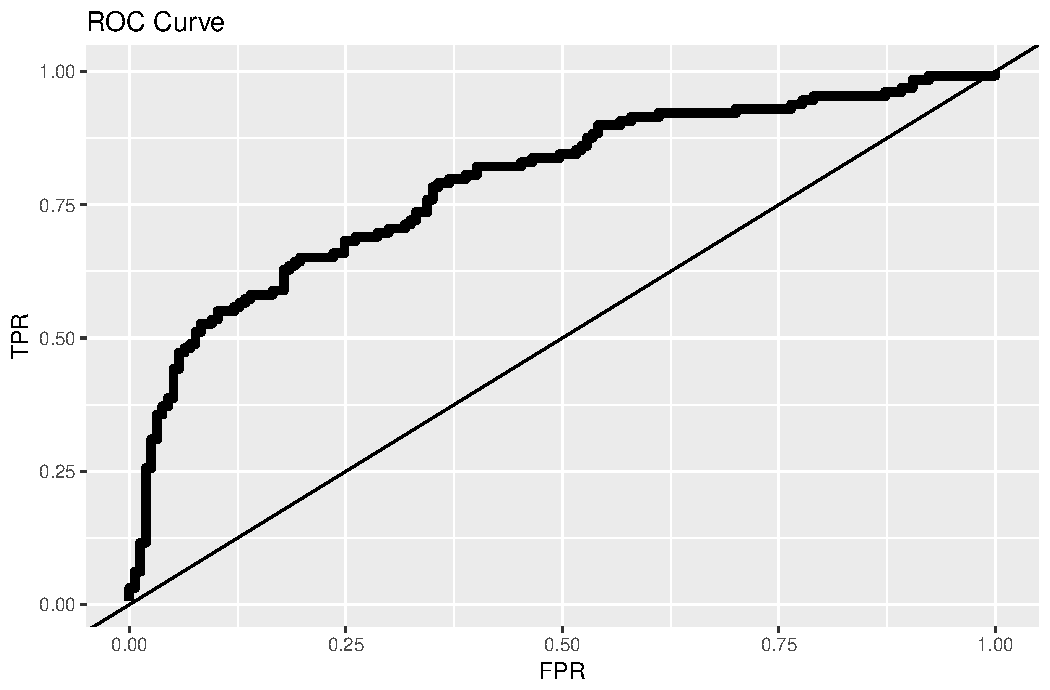
\includegraphics[width=0.8\textwidth]{usecase_pdf_files/figure-latex/unnamed-chunk-24-1} \end{center}

\subsection{Continue and Reposition the
Training}\label{continue-and-reposition-the-training}

The fastest way to continuing the training is to use the
\texttt{setToIteration()} function. If we set the algorithm to an
iteration bigger than the actual maximal iteration, then
\texttt{compboost} automatically trains the remaining baselearner:

\begin{Shaded}
\begin{Highlighting}[]
\NormalTok{cboost}\OperatorTok{$}\KeywordTok{setToIteration}\NormalTok{(}\DataTypeTok{k =} \DecValTok{3000}\NormalTok{)}
\NormalTok{## }
\NormalTok{## Set to a iteration bigger than already trained. Train 500 additional baselearner.}
\NormalTok{cboost}
\NormalTok{## }
\NormalTok{## Compboost object with:}
\NormalTok{##  - Learning Rate: 0.05}
\NormalTok{##  - Are all logger used as stopper: 0}
\NormalTok{##  - Model is already trained with 3000 iterations/fitted baselearner}
\NormalTok{##  - Actual state is at iteration 3000}
\NormalTok{##  - Loss optimal initialization: -0.25}
\NormalTok{## }
\NormalTok{## To get more information check the other objects!}
\end{Highlighting}
\end{Shaded}

The drawback of using \texttt{setToIteration()} is, that the function
doesn't continuing logging. The logger data for the second training
(from iteration 501 to 1000) is then just a vector of the iterations.

Additionally, it is possible to continuing the training using the
\texttt{continueTraining()} function. This function takes a boolian to
indicate if the trace should be printed and another logger list to get
more control about the retraining. For instance, we can continuing the
training for 3 seconds and see how far we get. We also want to reuse the
out of bag logger:

\begin{Shaded}
\begin{Highlighting}[]
\CommentTok{# Define new time logger:}
\NormalTok{new.time.logger =}\StringTok{ }\NormalTok{TimeLogger}\OperatorTok{$}\KeywordTok{new}\NormalTok{(}\DataTypeTok{use_as_stopper =} \OtherTok{TRUE}\NormalTok{, }\DataTypeTok{max_time =} \DecValTok{3}\NormalTok{,}
  \DataTypeTok{time_unit =} \StringTok{"seconds"}\NormalTok{)}

\CommentTok{# Define new logger list and register logger:}
\NormalTok{new.logger.list =}\StringTok{ }\NormalTok{LoggerList}\OperatorTok{$}\KeywordTok{new}\NormalTok{()}

\CommentTok{# Define new oob logger to prevent old logger data from overwriting:}
\NormalTok{new.oob.log     =}\StringTok{ }\NormalTok{OobRiskLogger}\OperatorTok{$}\KeywordTok{new}\NormalTok{(}\DataTypeTok{use_as_stopper =} \OtherTok{FALSE}\NormalTok{, }\DataTypeTok{used_loss =}\NormalTok{ loss.bin,}
  \DataTypeTok{eps_for_break =} \FloatTok{0.05}\NormalTok{, }\DataTypeTok{oob_data =}\NormalTok{ oob.list, }\DataTypeTok{oob_response =}\NormalTok{ response[idx.eval])}
\NormalTok{new.oob.auc.log =}\StringTok{ }\NormalTok{OobRiskLogger}\OperatorTok{$}\KeywordTok{new}\NormalTok{(}\DataTypeTok{use_as_stopper =} \OtherTok{FALSE}\NormalTok{, }\DataTypeTok{used_loss =}\NormalTok{ auc.loss,}
  \DataTypeTok{eps_for_break =} \FloatTok{0.05}\NormalTok{, }\DataTypeTok{oob_data =}\NormalTok{ oob.list, }\DataTypeTok{oob_response =}\NormalTok{ response[idx.eval])}

\NormalTok{new.logger.list}\OperatorTok{$}\KeywordTok{registerLogger}\NormalTok{(}\StringTok{"time"}\NormalTok{, new.time.logger)}
\NormalTok{new.logger.list}\OperatorTok{$}\KeywordTok{registerLogger}\NormalTok{(}\StringTok{"oob.binomial"}\NormalTok{, new.oob.log)}
\NormalTok{new.logger.list}\OperatorTok{$}\KeywordTok{registerLogger}\NormalTok{(}\StringTok{"oob.auc"}\NormalTok{, new.oob.auc.log)}

\CommentTok{# Continue training:}
\NormalTok{cboost}\OperatorTok{$}\KeywordTok{continueTraining}\NormalTok{(}\DataTypeTok{trace =} \OtherTok{FALSE}\NormalTok{, }\DataTypeTok{logger_list =}\NormalTok{ new.logger.list)}
\NormalTok{cboost}
\NormalTok{## }
\NormalTok{## Compboost object with:}
\NormalTok{##  - Learning Rate: 0.05}
\NormalTok{##  - Are all logger used as stopper: 0}
\NormalTok{##  - Model is already trained with 11954 iterations/fitted baselearner}
\NormalTok{##  - Actual state is at iteration 11954}
\NormalTok{##  - Loss optimal initialization: -0.25}
\NormalTok{## }
\NormalTok{## To get more information check the other objects!}
\end{Highlighting}
\end{Shaded}

Note: With \texttt{setToIteration()} it is also possible to set
\texttt{compboost} to an iteration smaller than the already trained
ones. This becomes handy if one would like set the algorithm to an
iteration corresponding to the minimum of the out of bag risk.

\subsection{Illustrating some Results}\label{illustrating-some-results}

\subsubsection{Inbag vs OOB}\label{inbag-vs-oob}

To compare the inbag and the out of bag AUC we first have to get the
logger data:

\begin{Shaded}
\begin{Highlighting}[]
\NormalTok{cboost.log =}\StringTok{ }\NormalTok{cboost}\OperatorTok{$}\KeywordTok{getLoggerData}\NormalTok{()}
\KeywordTok{str}\NormalTok{(cboost.log)}
\NormalTok{## List of 3}
\NormalTok{##  $ initial.training:List of 2}
\NormalTok{##   ..$ logger.names: chr [1:6] " iteration.logger" "inbag.auc" "inbag.binomial" "oob.auc" ...}
\NormalTok{##   ..$ logger.data : num [1:2500, 1:6] 1 2 3 4 5 6 7 8 9 10 ...}
\NormalTok{##  $ retraining1     :List of 2}
\NormalTok{##   ..$ logger.names: chr "setToIteration.retraining1"}
\NormalTok{##   ..$ logger.data : num [1:500, 1] 1 2 3 4 5 6 7 8 9 10 ...}
\NormalTok{##  $ retraining2     :List of 2}
\NormalTok{##   ..$ logger.names: chr [1:3] "oob.auc" "oob.binomial" "time"}
\NormalTok{##   ..$ logger.data : num [1:8954, 1:3] 0.296 0.597 0.542 0.68 0.618 ...}
\end{Highlighting}
\end{Shaded}

This list contains all the data collected while training and retraining.
Therefore, three list elements. We are interested in the first one:

\begin{Shaded}
\begin{Highlighting}[]
\NormalTok{cboost.log =}\StringTok{ }\NormalTok{cboost.log[[}\DecValTok{1}\NormalTok{]]}
\KeywordTok{str}\NormalTok{(cboost.log)}
\NormalTok{## List of 2}
\NormalTok{##  $ logger.names: chr [1:6] " iteration.logger" "inbag.auc" "inbag.binomial" "oob.auc" ...}
\NormalTok{##  $ logger.data : num [1:2500, 1:6] 1 2 3 4 5 6 7 8 9 10 ...}
\end{Highlighting}
\end{Shaded}

Next we create a data frame which we use for plotting:

\begin{Shaded}
\begin{Highlighting}[]
\NormalTok{auc.data =}\StringTok{ }\KeywordTok{data.frame}\NormalTok{(}
  \DataTypeTok{iteration =} \KeywordTok{rep}\NormalTok{(}\KeywordTok{seq_len}\NormalTok{(}\KeywordTok{nrow}\NormalTok{(cboost.log}\OperatorTok{$}\NormalTok{logger.data)), }\DecValTok{2}\NormalTok{),}
  \DataTypeTok{risk.type =} \KeywordTok{rep}\NormalTok{(}\KeywordTok{c}\NormalTok{(}\StringTok{"Inbag"}\NormalTok{, }\StringTok{"OOB"}\NormalTok{), }\DataTypeTok{each =} \KeywordTok{nrow}\NormalTok{(cboost.log}\OperatorTok{$}\NormalTok{logger.data)),}
  \DataTypeTok{AUC       =} \KeywordTok{c}\NormalTok{(cboost.log}\OperatorTok{$}\NormalTok{logger.data[, }\DecValTok{2}\NormalTok{], cboost.log}\OperatorTok{$}\NormalTok{logger.data[, }\DecValTok{4}\NormalTok{]),}
  \DataTypeTok{emp.risk  =} \KeywordTok{c}\NormalTok{(cboost.log}\OperatorTok{$}\NormalTok{logger.data[, }\DecValTok{3}\NormalTok{], cboost.log}\OperatorTok{$}\NormalTok{logger.data[, }\DecValTok{5}\NormalTok{])}
\NormalTok{)}

\NormalTok{p1 =}\StringTok{ }\KeywordTok{ggplot}\NormalTok{(}\DataTypeTok{data =}\NormalTok{ auc.data, }\KeywordTok{aes}\NormalTok{(}\DataTypeTok{x =}\NormalTok{ iteration, }\DataTypeTok{y =}\NormalTok{ AUC, }\DataTypeTok{colour =}\NormalTok{ risk.type)) }\OperatorTok{+}
\StringTok{  }\KeywordTok{geom_line}\NormalTok{(}\DataTypeTok{size =} \DecValTok{2}\NormalTok{) }\OperatorTok{+}
\StringTok{  }\KeywordTok{ggtitle}\NormalTok{(}\StringTok{"AUC per Iteration"}\NormalTok{)}

\NormalTok{p2 =}\StringTok{ }\KeywordTok{ggplot}\NormalTok{(}\DataTypeTok{data =}\NormalTok{ auc.data, }\KeywordTok{aes}\NormalTok{(}\DataTypeTok{x =}\NormalTok{ iteration, }\DataTypeTok{y =}\NormalTok{ emp.risk, }\DataTypeTok{colour =}\NormalTok{ risk.type)) }\OperatorTok{+}
\StringTok{  }\KeywordTok{geom_line}\NormalTok{(}\DataTypeTok{size =} \DecValTok{2}\NormalTok{) }\OperatorTok{+}
\StringTok{  }\KeywordTok{ggtitle}\NormalTok{(}\StringTok{"Empirical Risk per Iteration"}\NormalTok{)}

\NormalTok{gridExtra}\OperatorTok{::}\KeywordTok{grid.arrange}\NormalTok{(p1, p2, }\DataTypeTok{ncol =} \DecValTok{2}\NormalTok{)}
\end{Highlighting}
\end{Shaded}

\begin{center}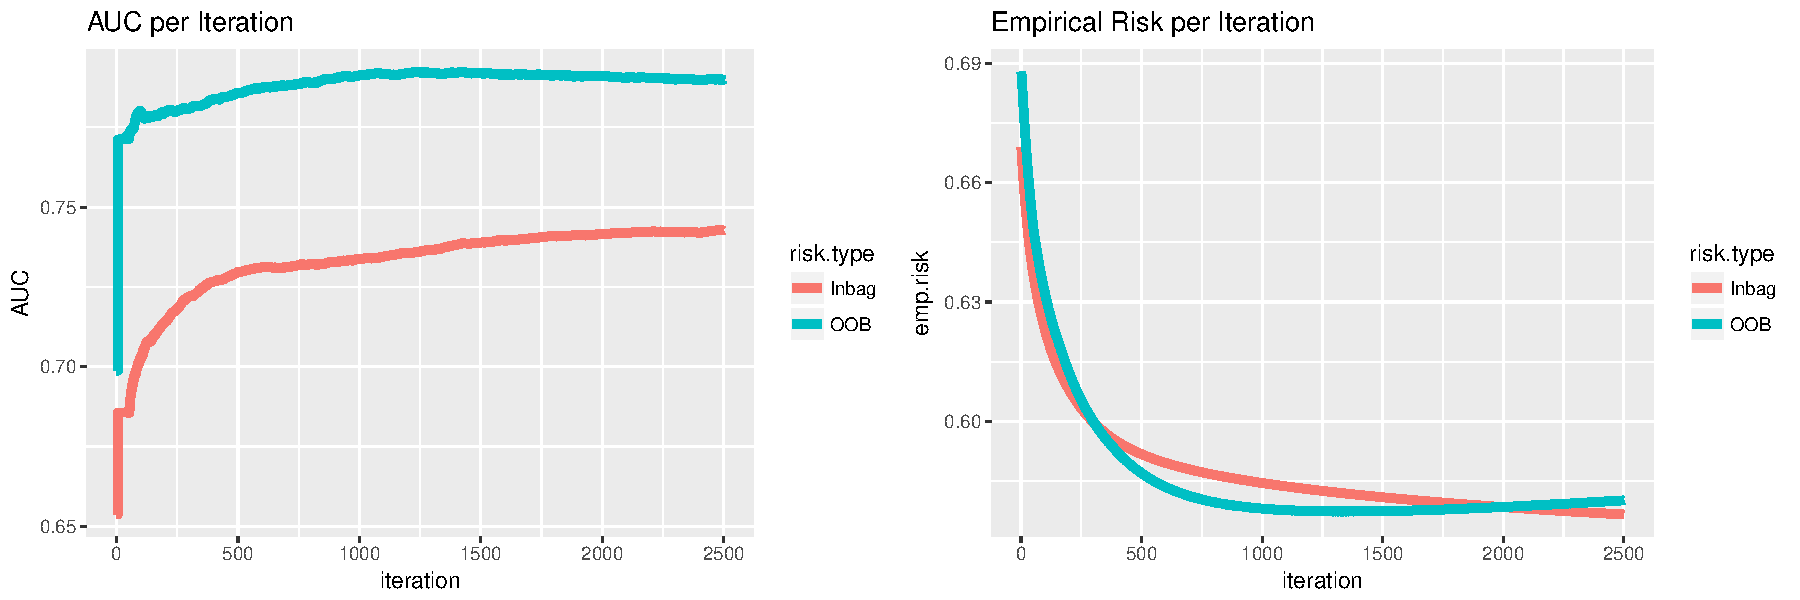
\includegraphics[width=0.8\textwidth]{usecase_pdf_files/figure-latex/unnamed-chunk-29-1} \end{center}

A surprising behavior is the AUC lines. We would expect the out of bag
AUC lower than the inbag AUC which isn't the case here. If we leave that
out the curves shows the usual behavior. The out of bag curve for the
AUC raises till approximately 1200 iterations and then decrease. On the
other hand, the out of bag risk also falls till approximately 1200 and
then starts to increase. This are clear signs that for more than 1200
iterations the algorithm starts to overfit. We should think about using
the model at the 1200th iteration.

\subsubsection{Fare Spline Baselearner}\label{fare-spline-baselearner}

One of the key advantages of component-wise boosting is to have an
interpretable model. For instance it is now possible to illustrate the
effect of fare. Therefore, we can use the \texttt{transformData()}
function of the \texttt{spline.factory.fare} object to create the spline
basis for new observations:

\begin{Shaded}
\begin{Highlighting}[]
\NormalTok{params =}\StringTok{ }\NormalTok{cboost}\OperatorTok{$}\KeywordTok{getEstimatedParameter}\NormalTok{()}
\NormalTok{params.fare =}\StringTok{ }\NormalTok{params}\OperatorTok{$}\StringTok{`}\DataTypeTok{Fare: spline with degree 3}\StringTok{`}

\NormalTok{x.fare  =}\StringTok{ }\KeywordTok{seq}\NormalTok{(}\DataTypeTok{from =} \KeywordTok{min}\NormalTok{(df.train}\OperatorTok{$}\NormalTok{Fare), }\DataTypeTok{to =} \KeywordTok{max}\NormalTok{(df.train}\OperatorTok{$}\NormalTok{Fare), }\DataTypeTok{length.out =} \DecValTok{100}\NormalTok{)}
\NormalTok{x.basis =}\StringTok{ }\NormalTok{spline.factory.fare}\OperatorTok{$}\KeywordTok{transformData}\NormalTok{(}\KeywordTok{as.matrix}\NormalTok{(x.fare))}
\NormalTok{x.response =}\StringTok{ }\NormalTok{x.basis }\OperatorTok\StringTok{ }\NormalTok{params.fare}

\NormalTok{plot.data =}\StringTok{ }\KeywordTok{data.frame}\NormalTok{(}\DataTypeTok{x =}\NormalTok{ x.fare, }\DataTypeTok{y =} \KeywordTok{as.numeric}\NormalTok{(x.response))}

\KeywordTok{ggplot}\NormalTok{(}\DataTypeTok{data =}\NormalTok{ plot.data, }\KeywordTok{aes}\NormalTok{(}\DataTypeTok{x =}\NormalTok{ x, }\DataTypeTok{y =}\NormalTok{ y)) }\OperatorTok{+}
\StringTok{  }\KeywordTok{geom_line}\NormalTok{(}\DataTypeTok{size =} \DecValTok{2}\NormalTok{) }\OperatorTok{+}
\StringTok{  }\KeywordTok{xlab}\NormalTok{(}\StringTok{"Ticket Costs (Fare)"}\NormalTok{) }\OperatorTok{+}
\StringTok{  }\KeywordTok{ylab}\NormalTok{(}\StringTok{"Additive Contribution"}\NormalTok{) }\OperatorTok{+}
\StringTok{  }\KeywordTok{labs}\NormalTok{(}\DataTypeTok{title=}\StringTok{"Effect of Age on Survival"}\NormalTok{, }
       \DataTypeTok{subtitle=}\StringTok{"The higher the additive contribution the higher the chance of survial"}\NormalTok{)}
\end{Highlighting}
\end{Shaded}

\begin{center}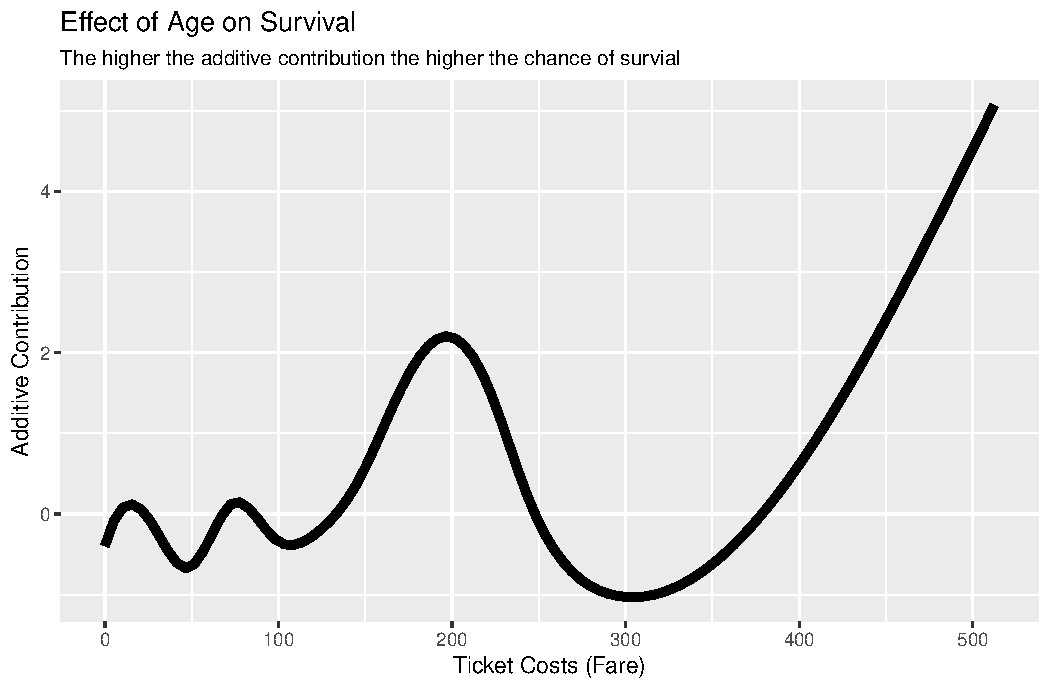
\includegraphics[width=0.8\textwidth]{usecase_pdf_files/figure-latex/unnamed-chunk-30-1} \end{center}

We recognize, that this curve results from taking the parameter after
11954 iterations. That could be way too much and could tend to
overfitting. Because of the out of bag behavior, we set the iteration to
1200:

\begin{Shaded}
\begin{Highlighting}[]
\NormalTok{cboost}\OperatorTok{$}\KeywordTok{setToIteration}\NormalTok{(}\DataTypeTok{k =} \DecValTok{1200}\NormalTok{)}

\NormalTok{params =}\StringTok{ }\NormalTok{cboost}\OperatorTok{$}\KeywordTok{getEstimatedParameter}\NormalTok{()}
\NormalTok{params.fare =}\StringTok{ }\NormalTok{params}\OperatorTok{$}\StringTok{`}\DataTypeTok{Fare: spline with degree 3}\StringTok{`}

\NormalTok{x.fare  =}\StringTok{ }\KeywordTok{seq}\NormalTok{(}\DataTypeTok{from =} \KeywordTok{min}\NormalTok{(df.train}\OperatorTok{$}\NormalTok{Fare), }\DataTypeTok{to =} \KeywordTok{max}\NormalTok{(df.train}\OperatorTok{$}\NormalTok{Fare), }\DataTypeTok{length.out =} \DecValTok{100}\NormalTok{)}
\NormalTok{x.basis =}\StringTok{ }\NormalTok{spline.factory.fare}\OperatorTok{$}\KeywordTok{transformData}\NormalTok{(}\KeywordTok{as.matrix}\NormalTok{(x.fare))}
\NormalTok{x.response =}\StringTok{ }\NormalTok{x.basis }\OperatorTok\StringTok{ }\NormalTok{params.fare}

\NormalTok{plot.data =}\StringTok{ }\KeywordTok{data.frame}\NormalTok{(}\DataTypeTok{x =}\NormalTok{ x.fare, }\DataTypeTok{y =} \KeywordTok{as.numeric}\NormalTok{(x.response))}

\KeywordTok{ggplot}\NormalTok{(}\DataTypeTok{data =}\NormalTok{ plot.data, }\KeywordTok{aes}\NormalTok{(}\DataTypeTok{x =}\NormalTok{ x, }\DataTypeTok{y =}\NormalTok{ y)) }\OperatorTok{+}
\StringTok{  }\KeywordTok{geom_line}\NormalTok{(}\DataTypeTok{size =} \DecValTok{2}\NormalTok{) }\OperatorTok{+}
\StringTok{  }\KeywordTok{xlab}\NormalTok{(}\StringTok{"Ticket Costs (Fare)"}\NormalTok{) }\OperatorTok{+}
\StringTok{  }\KeywordTok{ylab}\NormalTok{(}\StringTok{"Additive Contribution"}\NormalTok{) }\OperatorTok{+}
\StringTok{  }\KeywordTok{labs}\NormalTok{(}\DataTypeTok{title=}\StringTok{"Effect of Age on Survival"}\NormalTok{, }
       \DataTypeTok{subtitle=}\StringTok{"The higher the additive contribution the higher the chance of survial"}\NormalTok{)}
\end{Highlighting}
\end{Shaded}

\begin{center}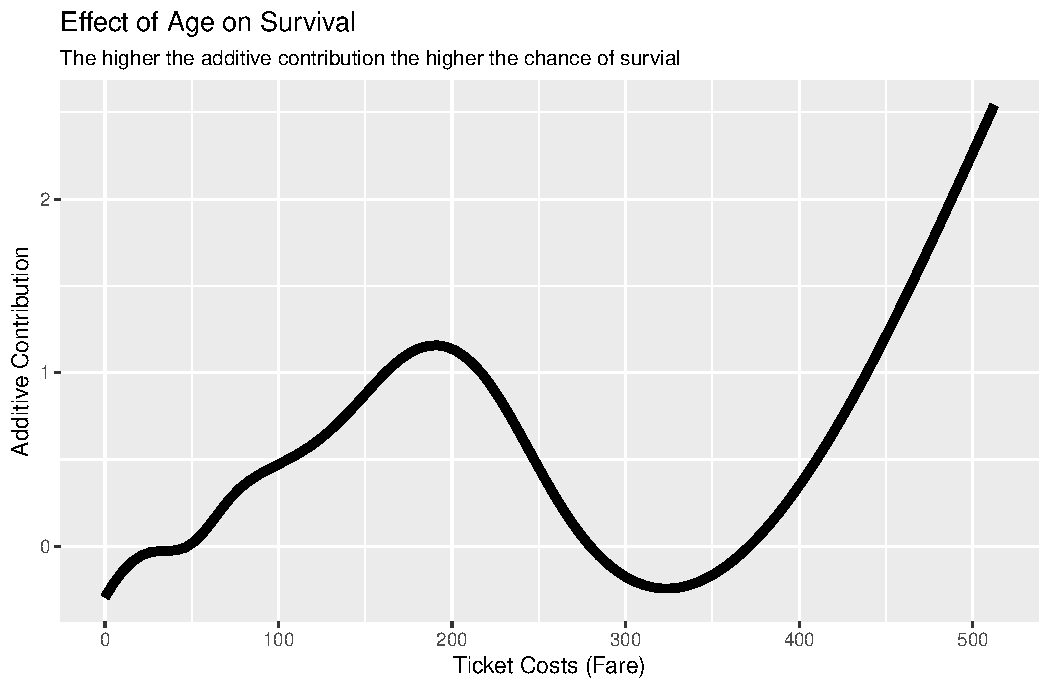
\includegraphics[width=0.8\textwidth]{usecase_pdf_files/figure-latex/unnamed-chunk-31-1} \end{center}

\subsection{Some Remarks}\label{some-remarks}

\begin{itemize}
\item
  We know that define everything using the \texttt{C++} class style is
  very odd, but it reflects best the underlying \texttt{C++} class
  system. Additionally, using the class system gives the user maximal
  flexibility and control about the algorithm. An \texttt{R} API which
  looks more familiar to the most users is in progress and one of the
  most important next task.
\item
  All the sample analyses we have made here are just to give an idea how
  \texttt{compboost} can be used to train a component-wise boosting
  model and how to access the data which are gained while the fitting
  process.
\item
  Since \texttt{compboost} is in an very early stage, the functionality
  isn't very comprehensive. For instance there is just one optimizer at
  the moment and one loss class for binary classification. There is also
  no multiclass support at the moment.
\item
  If someone wants to use a custom loss or baselearner we have
  implemented ways to extend compboost without recompiling the
  \texttt{C++} code. Therefore see the \href{}{extending compboost
  vignette}.
\end{itemize}

\subsection*{References}\label{references}
\addcontentsline{toc}{subsection}{References}

\hypertarget{refs}{}
\hypertarget{ref-eddelbuettel2017exposing}{}
Eddelbuettel, Dirk, and Romain François. 2018. ``Exposing C++ Functions
and Classes with Rcpp Modules.'' \emph{Vignette Included in R Package
Rcpp, URL Http://CRAN. R-Project. Org/Package= Rcpp}. Citeseer.

\hypertarget{ref-hofner2011framework}{}
Hofner, Benjamin, Torsten Hothorn, Thomas Kneib, and Matthias Schmid.
2011. ``A Framework for Unbiased Model Selection Based on Boosting.''
\emph{Journal of Computational and Graphical Statistics} 20 (4). Taylor
\& Francis: 956--71.


\end{document}
